\section{Introduction}

% Need to define `theoretical resource assessment'

This paper has two primary objectives: 1) to define a new methodology for quantifying theoretical wave resource that addresses critiques of previous approaches that can be applied at any scale, and 2) to apply that method to all U.S. regions to obtain an updated assessment of the nation's wave energy potential (theoretical resource).

% Need to define:
% - "WEC"
% - "EPRI2011" (+ EPRI2004?)



\begin{figure}[ht]
  \centering
  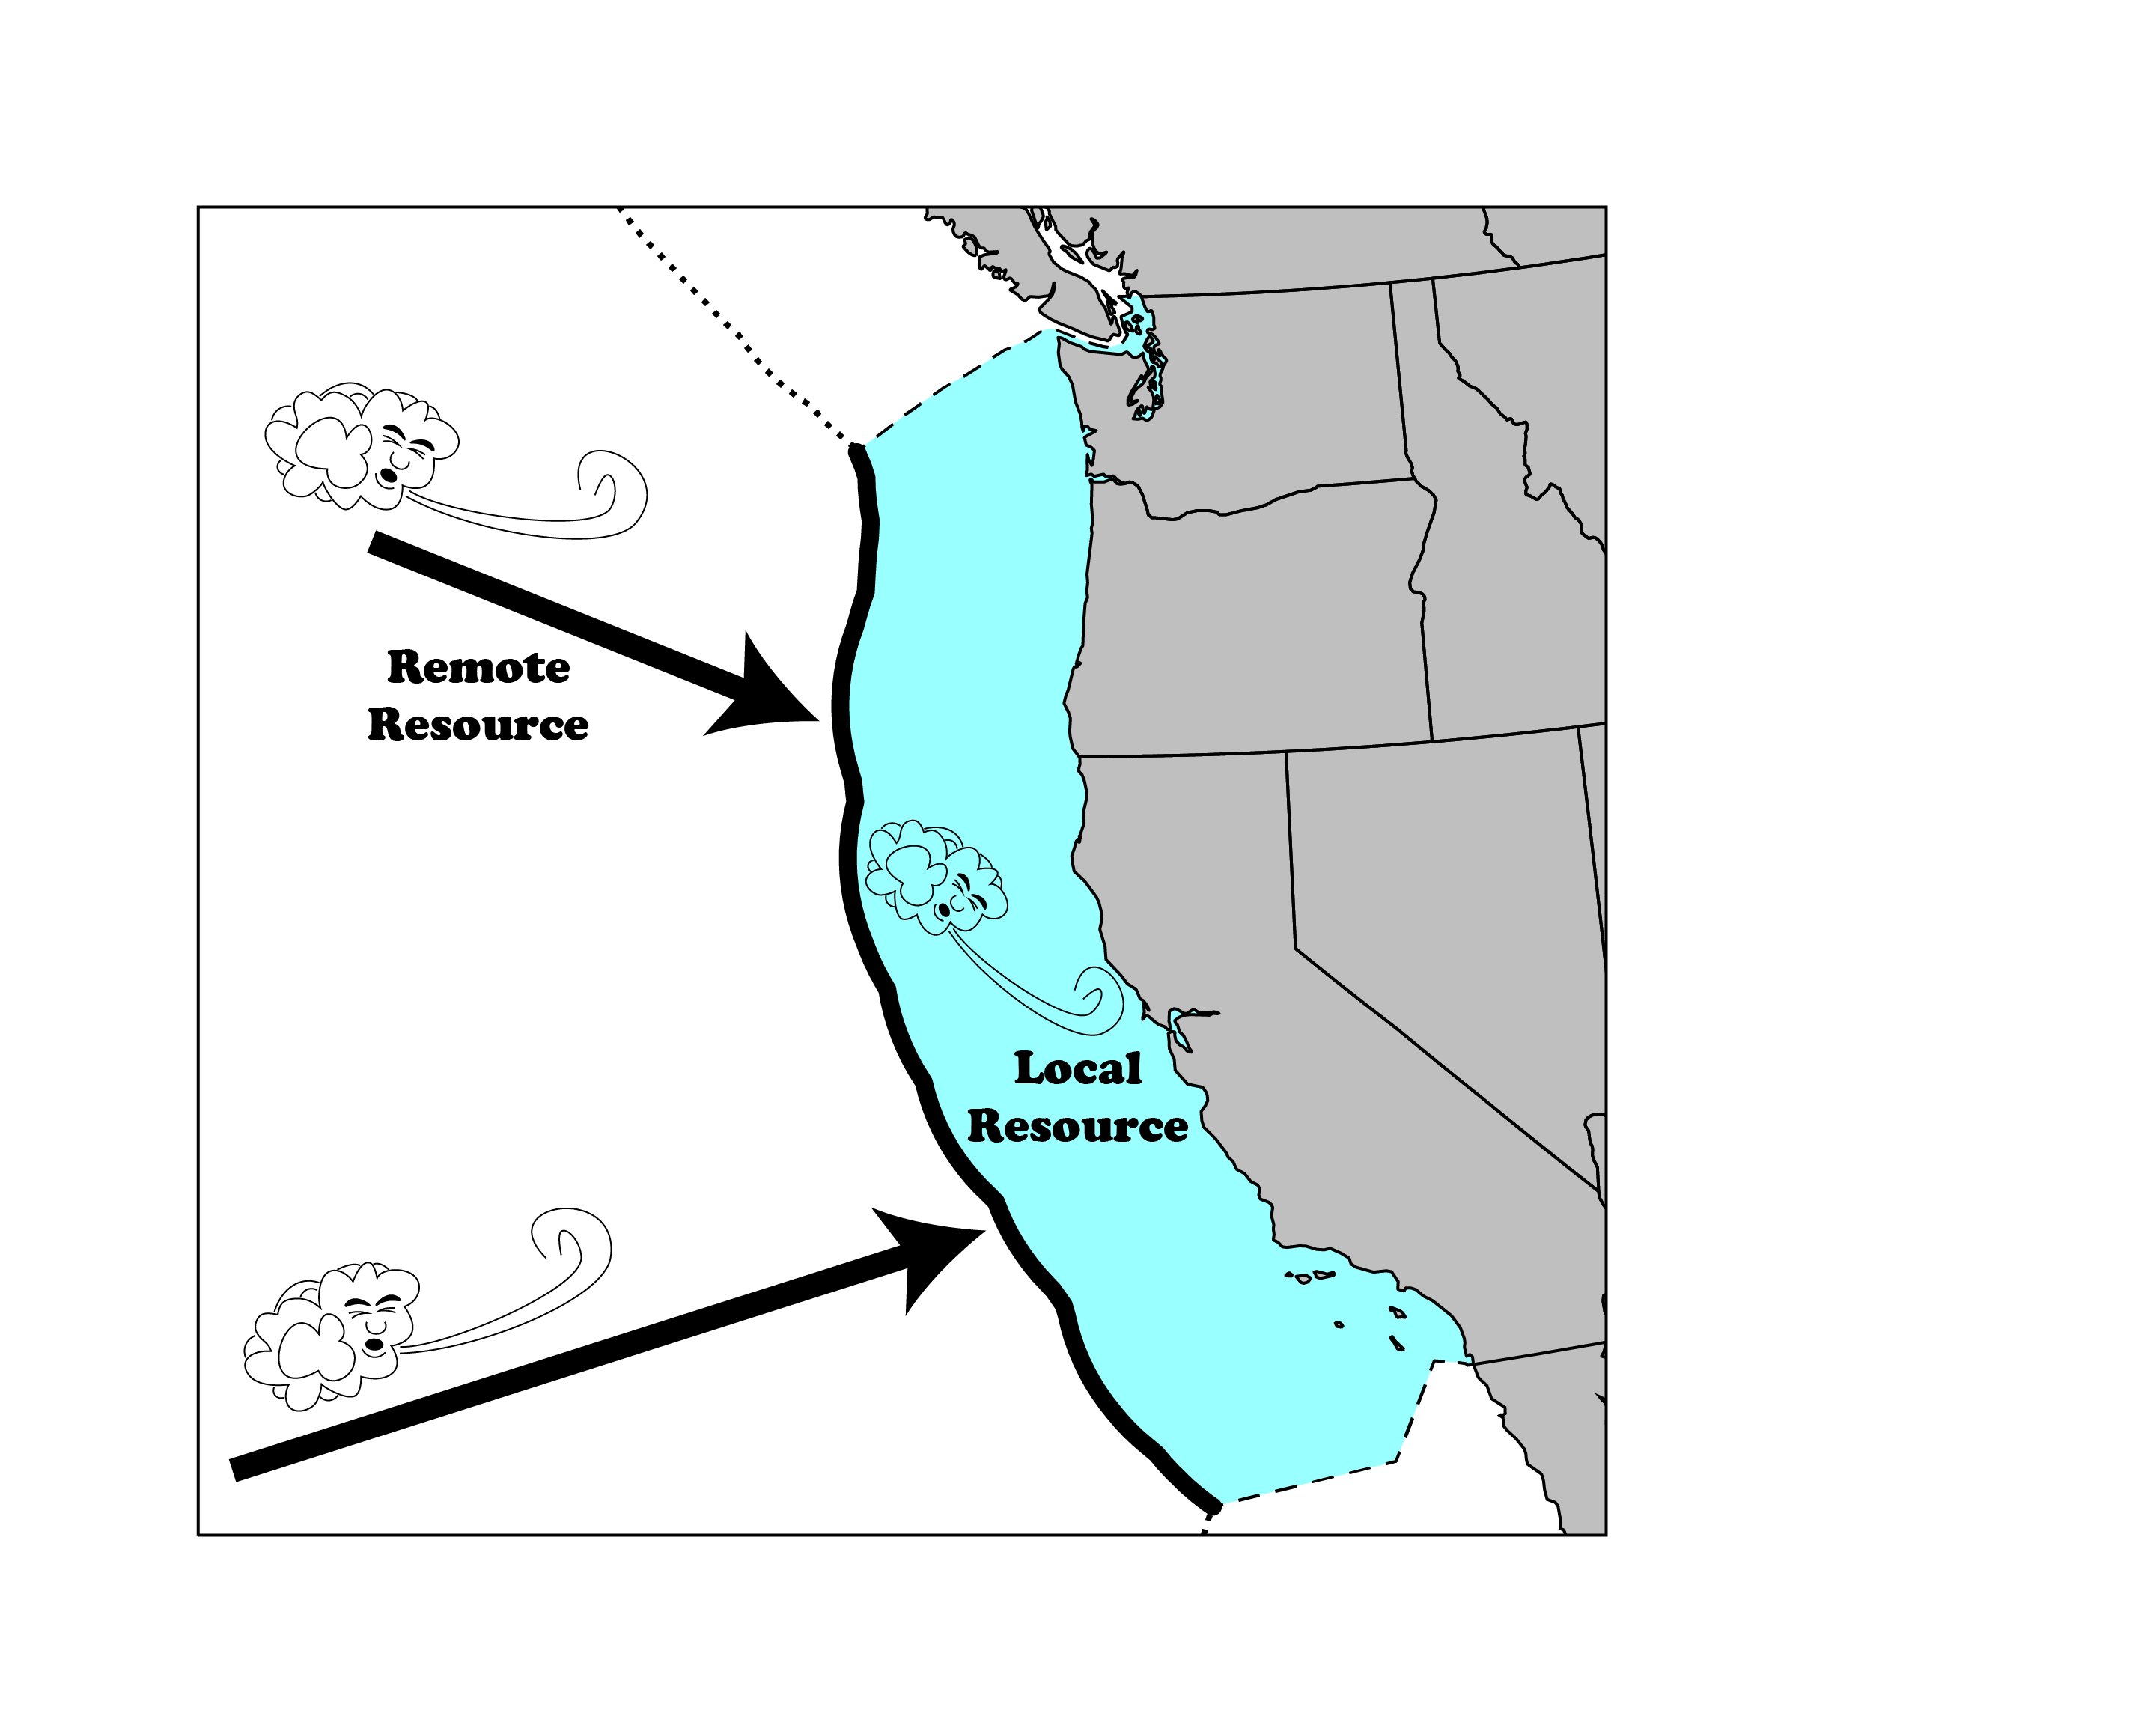
\includegraphics[width=0.9\linewidth]{../diagram/EEZ_contour03_edit01.png}
  \caption{A diagram depicting the U.S. West Coast’s ‘remote’ (arrows) and ‘local’ (cyan region) resource.}
  \label{fig:diagram:west-eez}
\end{figure}

The methodology developed here has been guided by the successes and limitations of previous works. In particular, several previous works have accurately quantified the remote resource, while others have utilized approaches that have been criticized for 'double counting'. Those works have shot back that, "sure, but you're not accounting for local winds".
\note{How to say this more tactfully?}


%%% Local Variables:
%%% TeX-master: "wave_res"
%%% End:
